\chapter{Instruction-Level Parallelism}
\label{chap:ilp}
Increasing processor performance has been provided by increased Instruction Level Parallelism (ILP). Processors have progressed from non-pipelined processors to pipelined processors to multiple pipeline processors to VLIW processors to superscalar processors; each step offers additional parallelism in the execution process.

Consider the following code fragment:
\begin{lstlisting}{asm}
mul r3, r4 -> r8
add r1, r2 -> r7
load r6, (r1)
add #5, r5
\end{lstlisting}

None of these instructions have dependencies on each other; that is, they are all independent. This means they can be executed in any order, and the CPU can rearrange them for the most performant execution order. Why does execution order matter? ILP allows you to execute multiple instructions at once, either through pipelining or through VLIW/superscalar approaches.

\section{Pipelining}
\begin{figure}
\centering
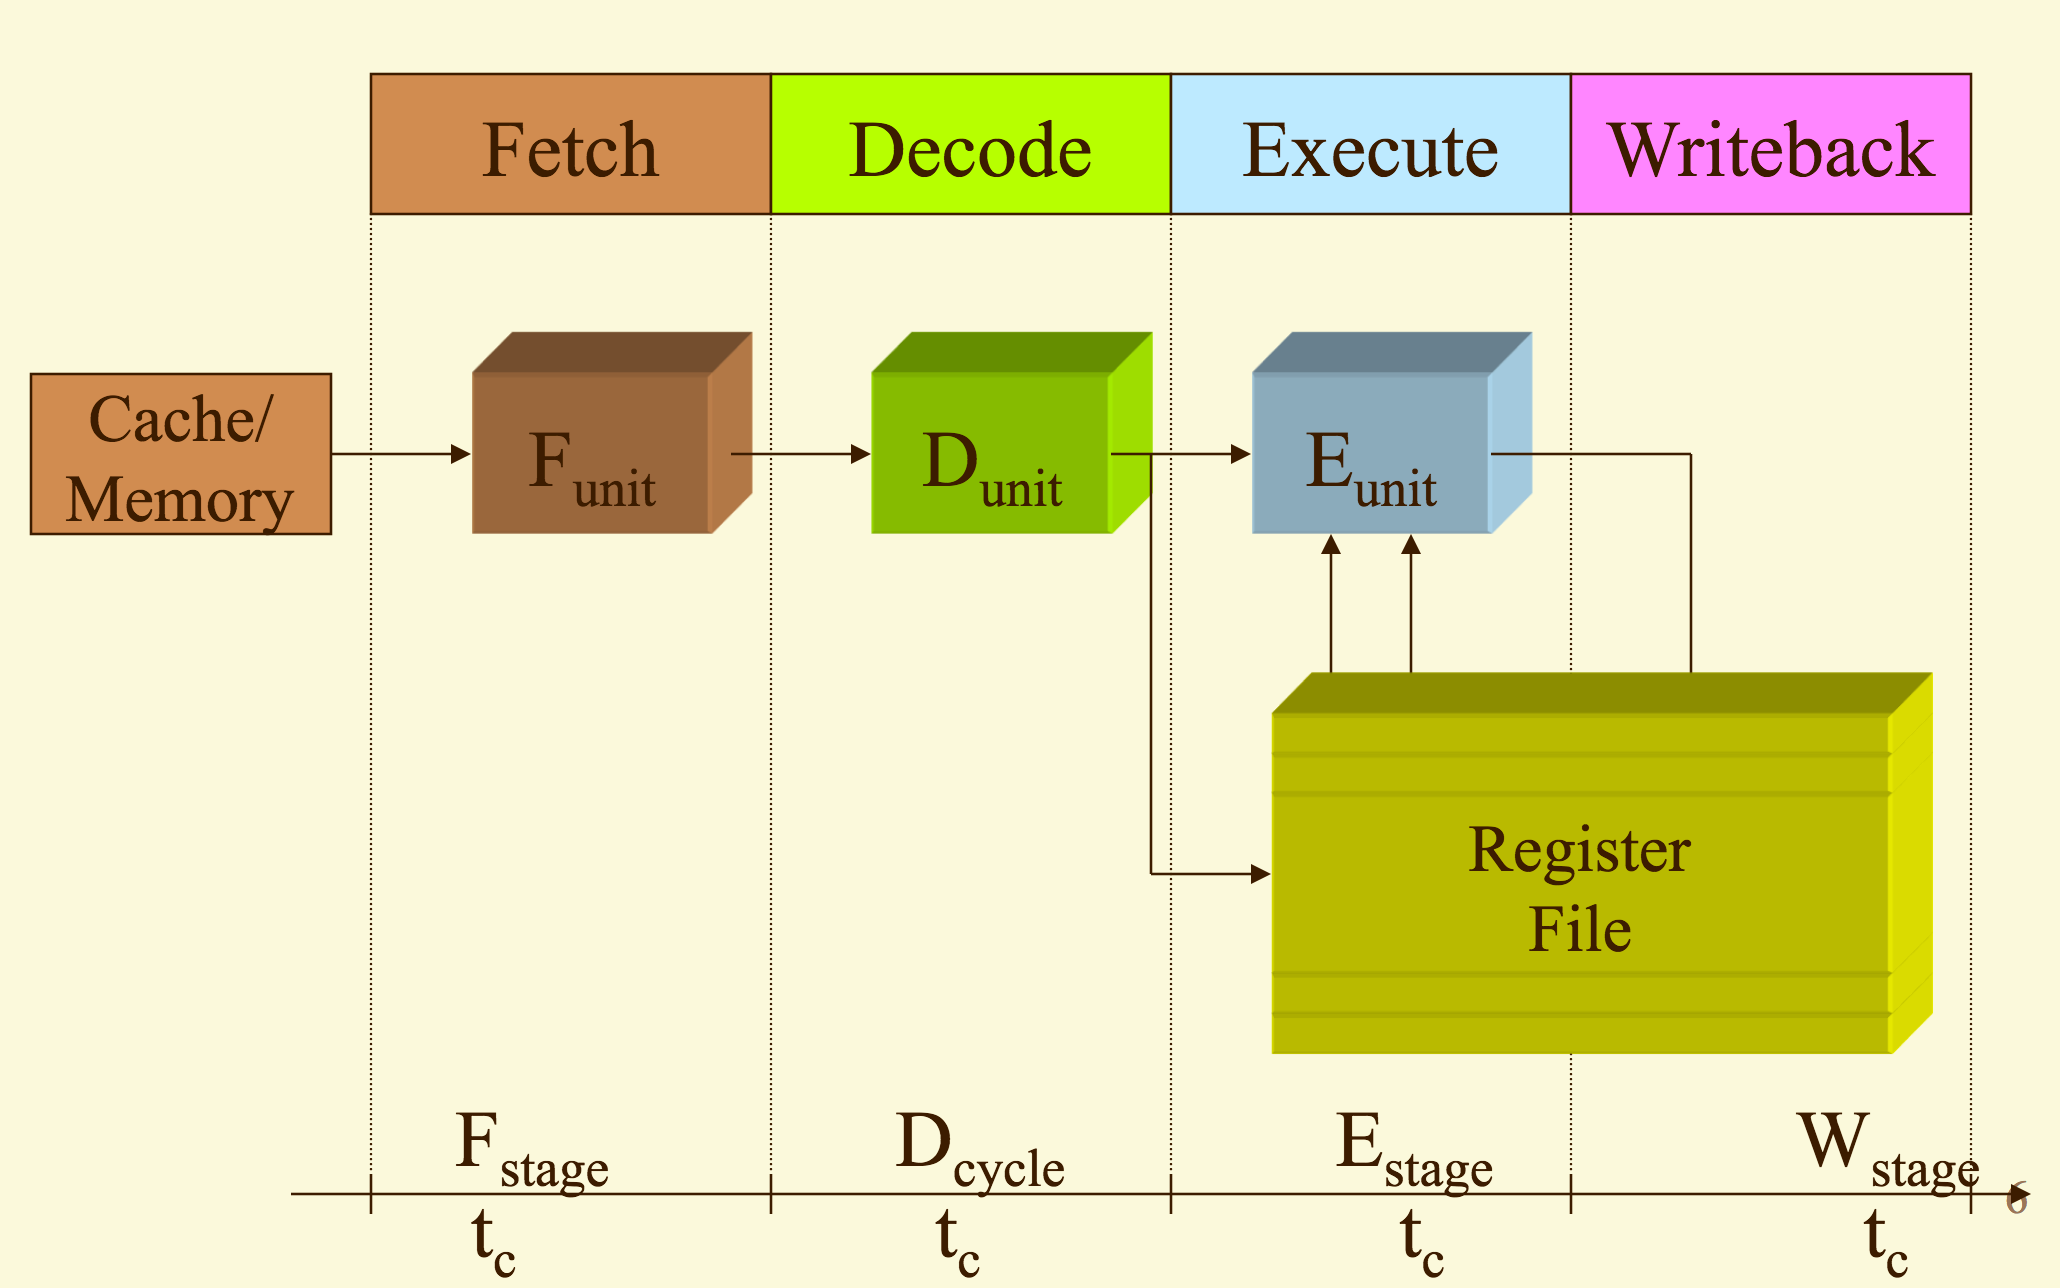
\includegraphics[width=0.7\linewidth]{figures/screenshot065}
\caption{Pipelining: splitting one operation into multiple stages.}
\label{fig:screenshot065}
\end{figure}

As seen in \autoref{fig:screenshot065}, operations can be split into multiple stages: fetch, decode, execute, and writeback. These are the typical stages, but more are possible; the Intel NetBurst architecture was infamous for having 31 stages in its pipeline. When an instruction is executed, it is in one of the stages; the other stages are free for use. 

This allows multiple instructions to be run simultaneously if each instruction is using a different stage of the pipeline. If instruction 1 is currently in the write-back stage, then instructions 2-4 after it can use the execute, decode and fetch stages. This is illustrated in \autoref{fig:screenshot066}.

\begin{figure}
\centering
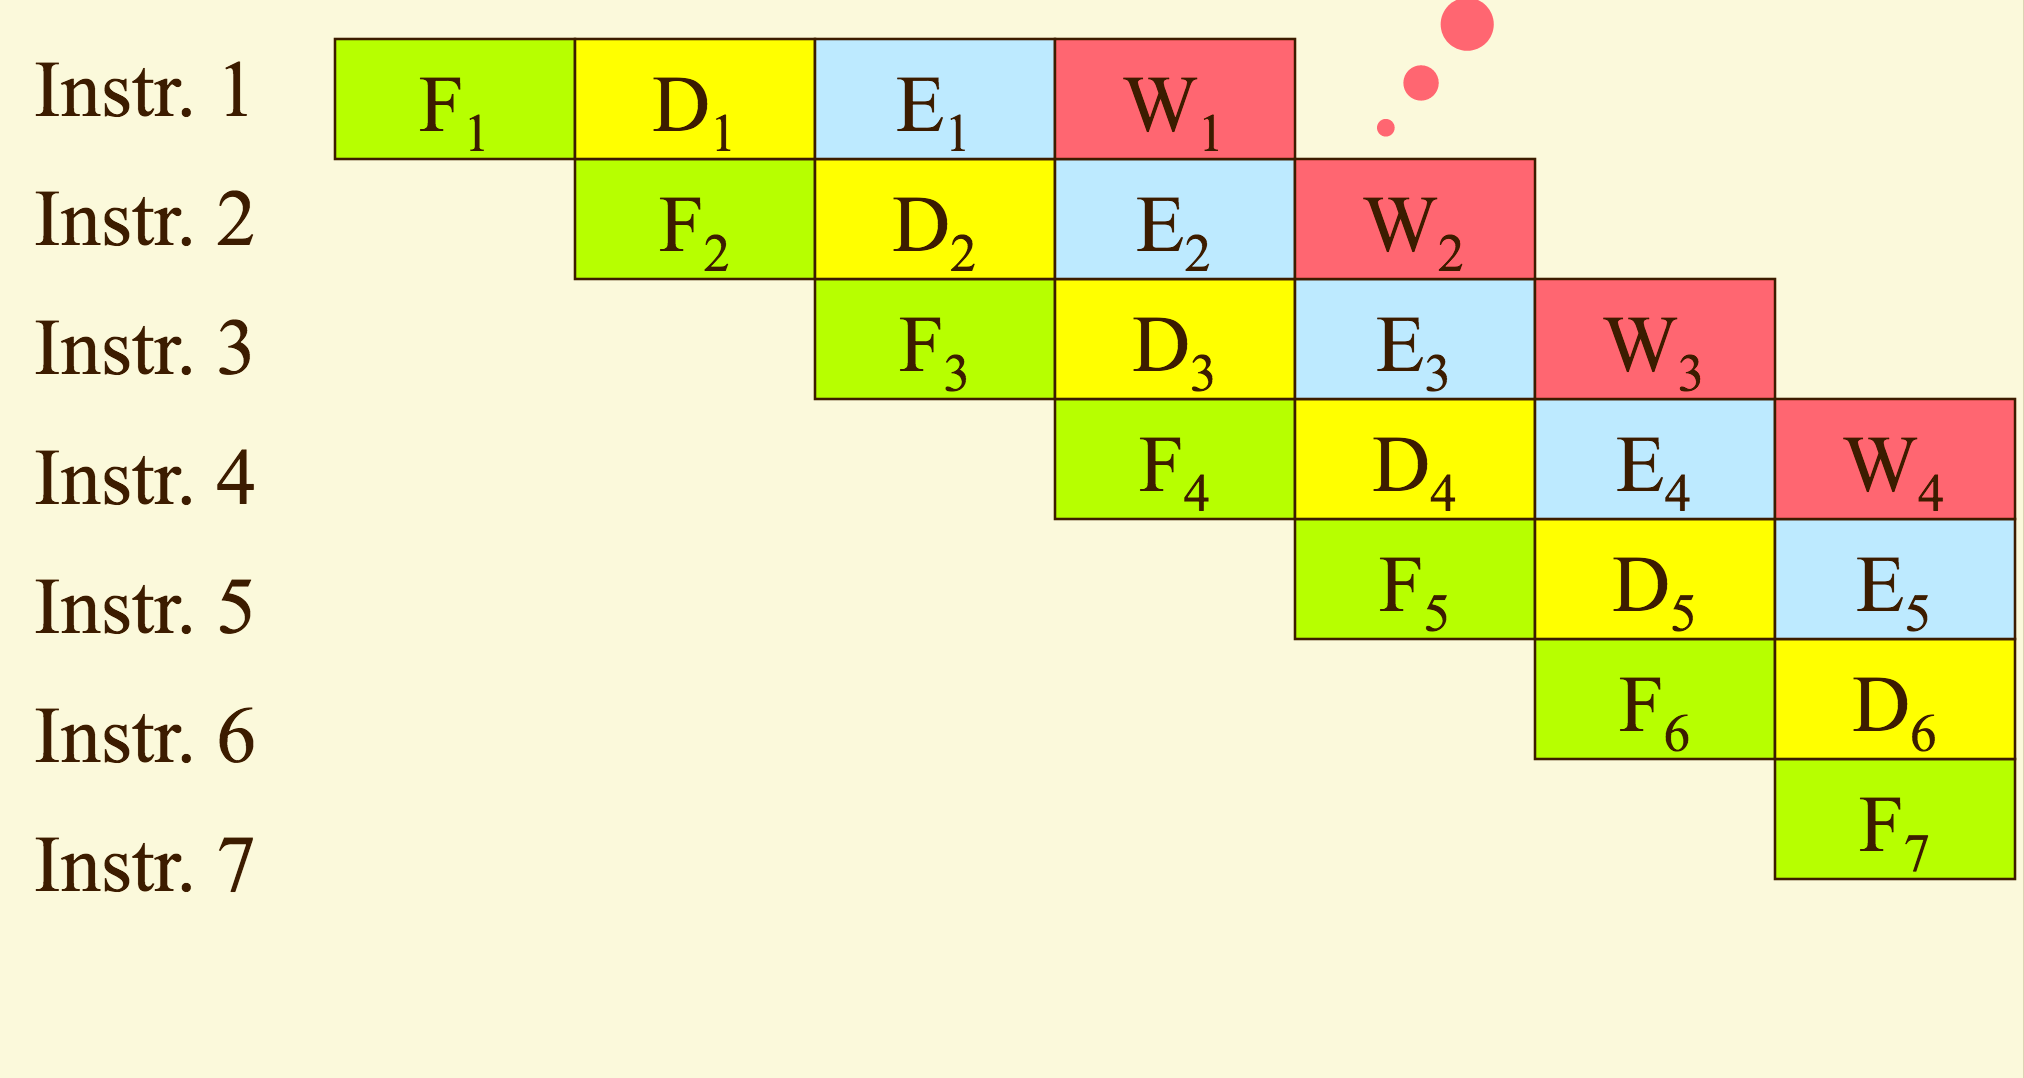
\includegraphics[width=0.7\linewidth]{figures/screenshot066}
\caption{Multiple instructions through pipelining.}
\label{fig:screenshot066}
\end{figure}

\section{VLIW/Superscalar}
Very Long Instruction Word (VLIW) and Superscalar approaches are largely similar. Essentially, there are multiple \textit{execution units} (EUs) dedicated to executing multiple instructions simultaneously. In VLIW, the instructions to be run across the units are scheduled in software (i.e. they are sequenced as part of the compiled machine code; see \autoref{fig:screenshot067}), while the superscalar approach is scheduled at runtime by the hardware (see \autoref{fig:screenshot068}).

\begin{figure}
\centering
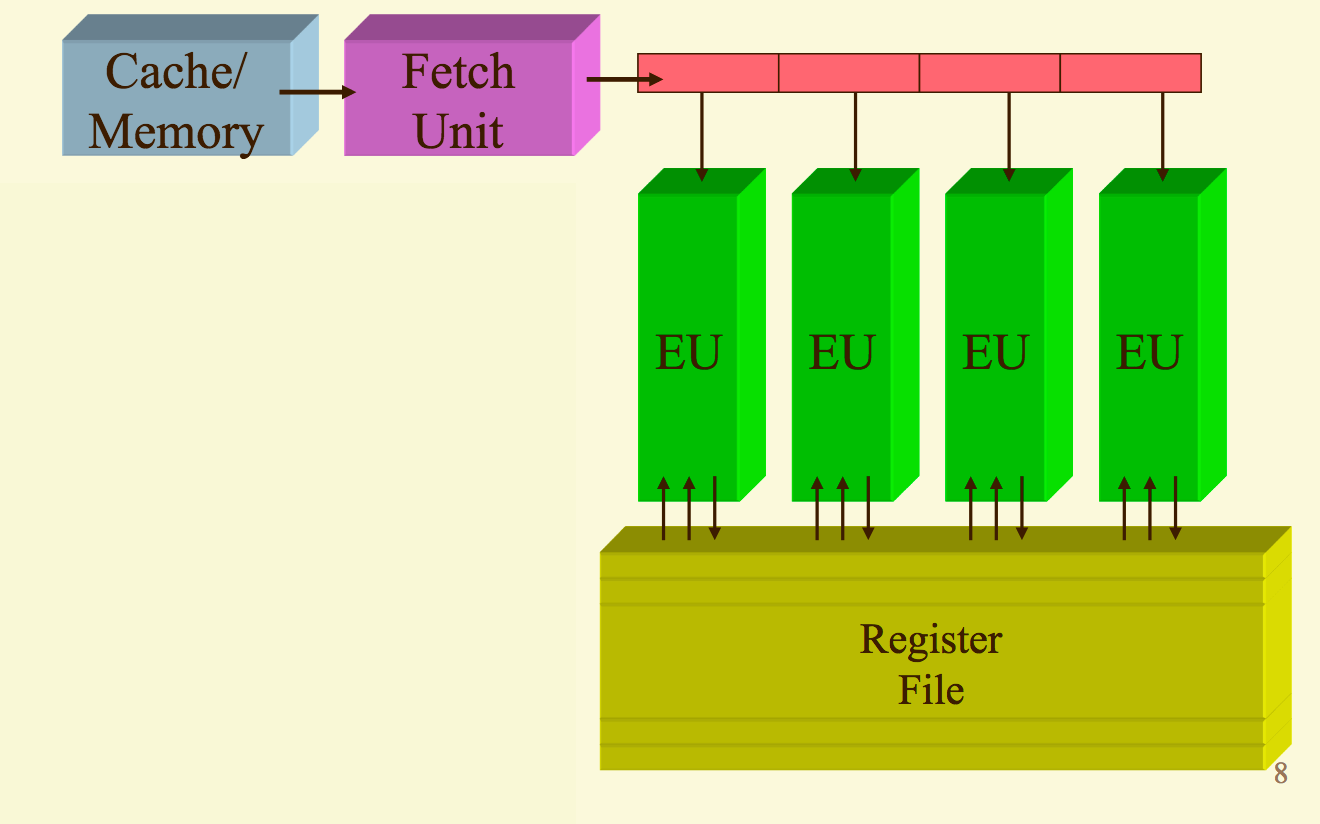
\includegraphics[width=0.7\linewidth]{figures/screenshot067}
\caption[VLIW approach.]{VLIW approach. Note how the four execution units are fed with the four segments of the one instruction word - you might even say the instruction word is \textit{very long}. The compiler decides which instructions form the instruction word at compile-time.}
\label{fig:screenshot067}
\end{figure}

\begin{figure}
\centering
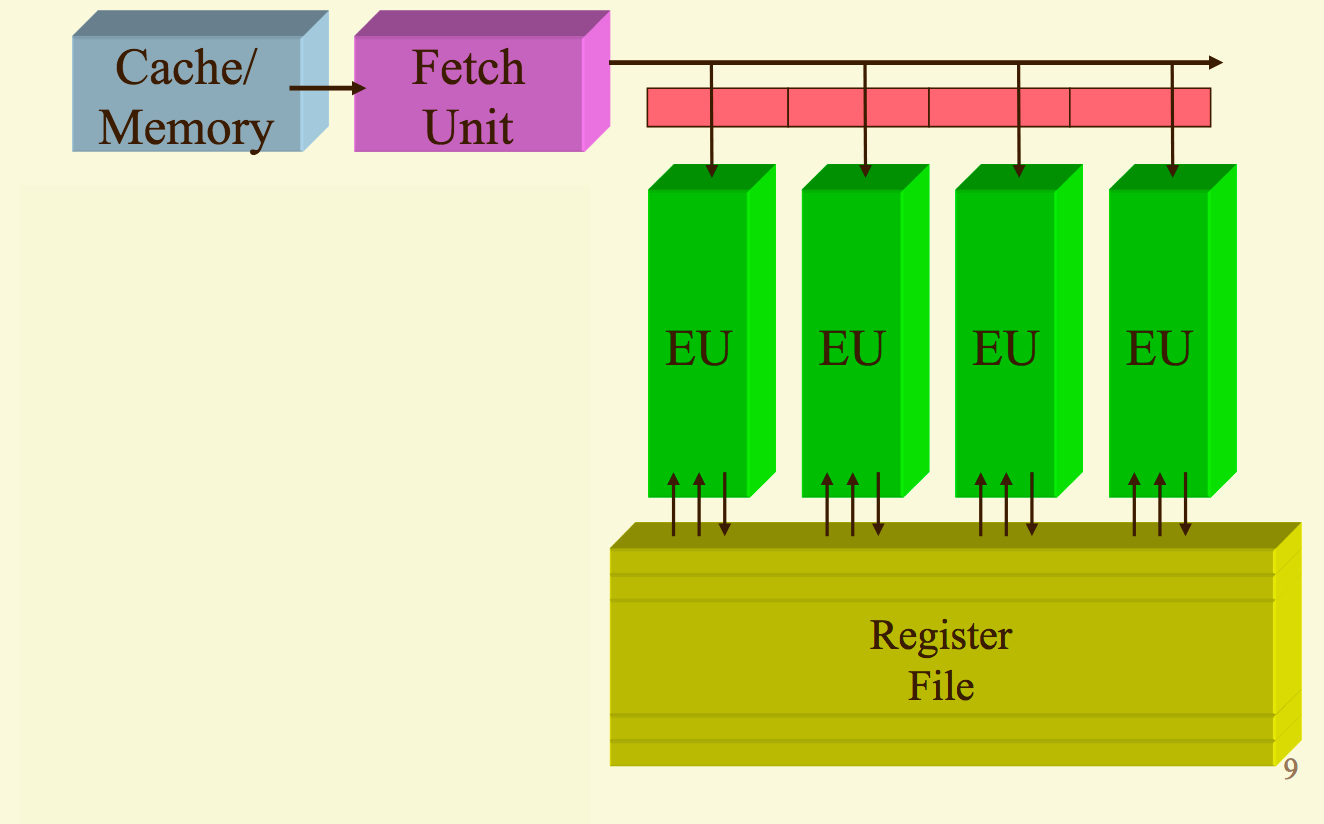
\includegraphics[width=0.7\linewidth]{figures/screenshot068}
\caption[Superscalar approach.]{Superscalar approach. There are four individual instructions that are concurrently fed to the execution units; the hardware is responsible for determining \textit{what} these four instructions are based on the instruction stream at runtime.}
\label{fig:screenshot068}
\end{figure}

\section{Dependencies}
\label{sec:dependencies}
However, in all instruction-level parallelism approaches, dependencies are a crucial factor. Dependencies are responsible for determining which instructions can be scheduled where, and whether they can be run in parallel or must be serialised.

There are multiple types of dependencies; these are discussed below.

\subsection{Data Dependencies}
Future instructions depend on the results of prior instructions; this means that future instructions have to wait on registers and memory to be resolved. These can be further broken down into two types of data dependencies: \begin{itemize}
\item \textbf{Read-after-write}: Data must be read, but is currently being written to. That is, if $r1$ is written to in instruction 1 and used in instruction 2, instruction 2 cannot be rearranged prior to instruction 1: it depends on the value written by instruction 1.

A load-use dependency is where a register is loaded from memory, and then used. A define-use dependency is where a register is assigned to by an instruction, and then used by another instruction.

\item \textbf{Write-after-read/write}: This is a \textit{false dependency}; it will result in the correct results as long as the instructions are executed in order. That is, a register that has been read/written to can be rewritten as long as the rewriting instruction occurs after the original read/write instruction. This can be broken by pipelining, but this can be fixed by using register renaming to temporarily change the registers being altered.
\end{itemize}

Not all data dependencies are obvious by examining the source code. As an example, a loop iteration that depends on the value calculated by the previous iteration has a data dependency; the compiler needs to be able to analyse loops to detect and handle these scenarios.

\subsection{Control Dependencies}
Future instructions cannot be evaluated until an upcoming branch in the instruction flow is evaluated - that is, code in an \texttt{if} branch can't normally be evaluated until the condition of the \texttt{if} has been evaluated.

This will normally stall a pipeline, unless special measures are taken (such as branch prediction). In general, for 25\% of code one in four instructions is a branch; as a result, control dependencies cannot be ignored. This is especially problematic for superscalar/VLIW architectures, where multiple EUs cannot be used to handle instructions that are blocked on a control dependency.

\subsection{Resource Dependencies}
The CPU has a limit to the number of Arithmetic Logic Units (ALUs), memory ports, and other resources at any given time; parallelism is fundamentally limited by the number of free resources.

\section{Scheduling}
There are three primary methods of instruction scheduling, briefly discussed prior.

\subsection{Static}
\begin{figure}
\centering
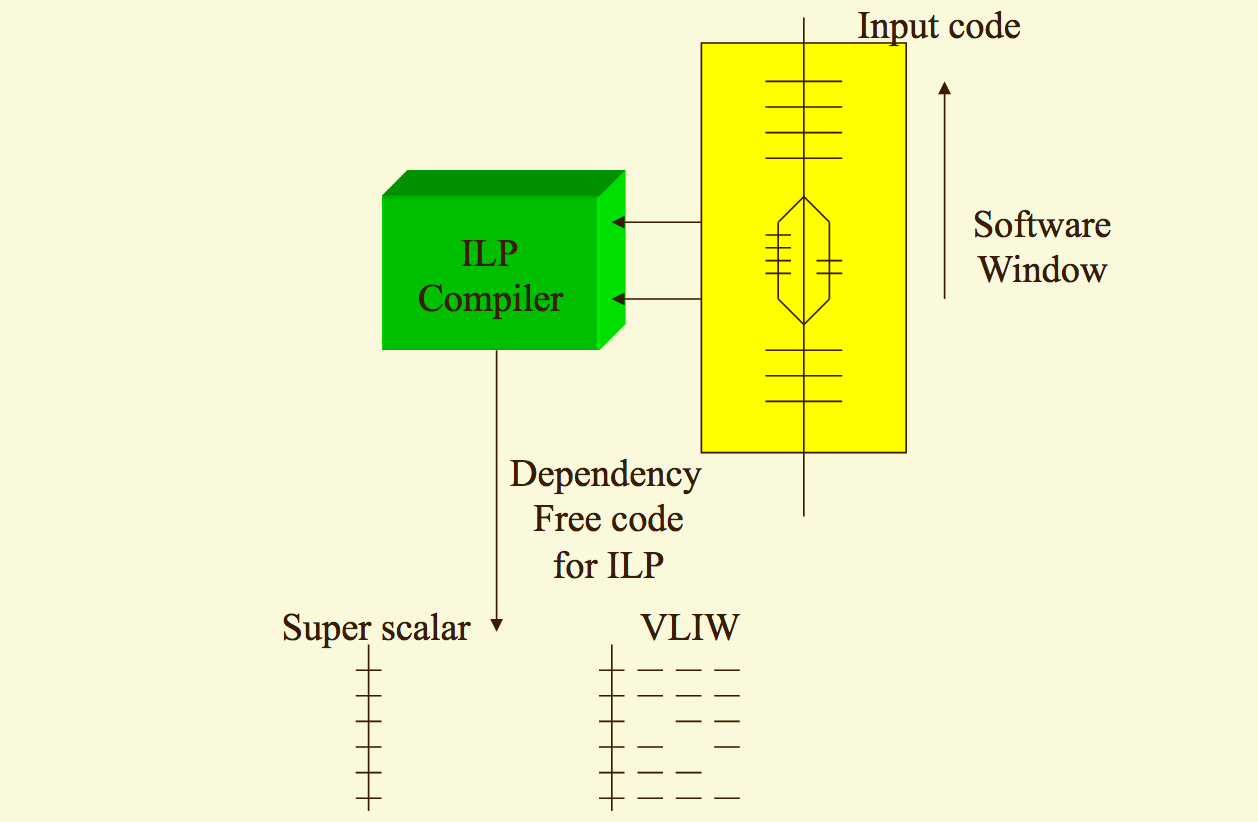
\includegraphics[width=0.7\linewidth]{figures/screenshot069}
\caption{Static scheduling.}
\label{fig:screenshot069}
\end{figure}

In static scheduling (depicted in \autoref{fig:screenshot069}), the compiler is responsible for generating optimal code that maximises instruction-level parallelism. The processor should receive dependency-free and optimised code for parallel execution. This is typical for VLIW architectures and a few pipelined processors (e.g. MIPS).

\subsection{Dynamic}
\begin{figure}
\centering
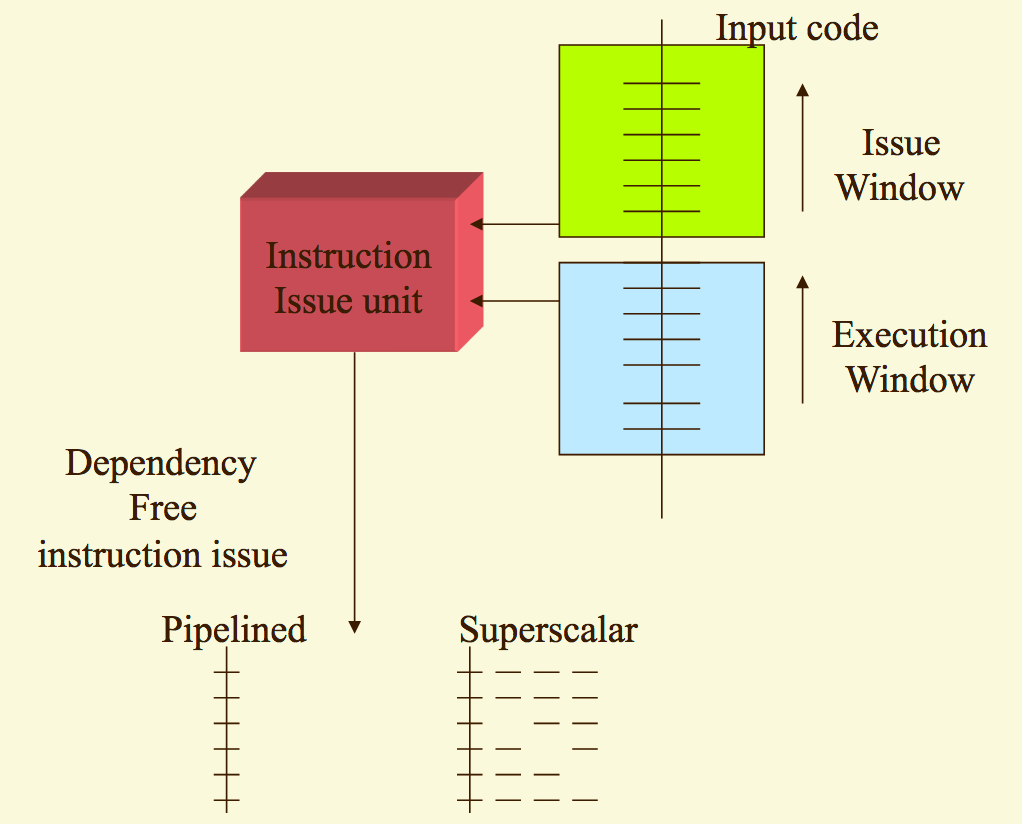
\includegraphics[width=0.7\linewidth]{figures/screenshot070}
\caption{Dynamic scheduling.}
\label{fig:screenshot070}
\end{figure}
In dynamic scheduling (depicted in \autoref{fig:screenshot070}), the hardware is responsible for determining the sequence of instructions in the incoming instruction stream that maximises instruction-level parallelism. It is performed entirely by the processor, which expects no effort on the behalf of the compiler to ease the scheduling problem. This was the approach favoured by early ILP processors (e.g. CDC 6600, IBM 360/91, and more).

\subsection{Hybrid}
In hybrid scheduling, both the compiler and the hardware work together to find optimal scheduling for instructions. The compiler makes a best-effort attempt to determine an appropriate scheduling; the hardware will then receive this, attempt to determine dependencies itself, and further optimise the instruction stream prior to execution. This is now commonplace, being the usual practice for modern pipelined superscalar processors (e.g. RS/6000, PL.8/XL, i960, QTC SF960, and notably modern x86 processors). 

\section{Sequential Consistency}
When instructions are executed in parallel, the processor must be careful to preserve sequential consistency of operations. Consider the following code:
\begin{lstlisting}{asm}
div r1, r2 -> r3
add r5, r6 -> r7
jz somewhere
\end{lstlisting}

The \texttt{div} and \texttt{add} set condition codes implicitly (in this case, whether or not the resulting value was zero), which are used by the \texttt{jz} instruction (which jumps when the if-zero condition code is set) to determine its next course of action. Division typically takes longer than addition; as a result, it is possible that the if-zero condition code of \texttt{div} may override that of \texttt{add}, despite \texttt{add} being evaluated "after" the \texttt{div}. Sequential consistency must be maintained to ensure that this is handled appropriately.

There are two kinds of consistency: \textit{strong consistency}, which preserves the actual execution order, and \textit{weak consistency}, which may execute out of order as long as the result is still correct.

\section{Performance}
The performance of instruction-level parallelism is fundamentally limited by \begin{itemize}
\item the underlying algorithm (which may have dependencies that cannot be removed)
\item compiled code (the compiler may introduce false dependencies and code that is difficult to pipeline)
\item actual hardware (the hardware may not have the resources to execute a given sequence of code in parallel)
\end{itemize}

All three of these factors must be considered when the maximum speedup is evaluated. Given this, previous studies have found potential speedups from the single-digits (i.e. 1.2 times faster) to hundreds of thousands of times faster (i.e. 64,500 times faster) for particular classes of applications on particular systems.

\begin{figure}
\centering
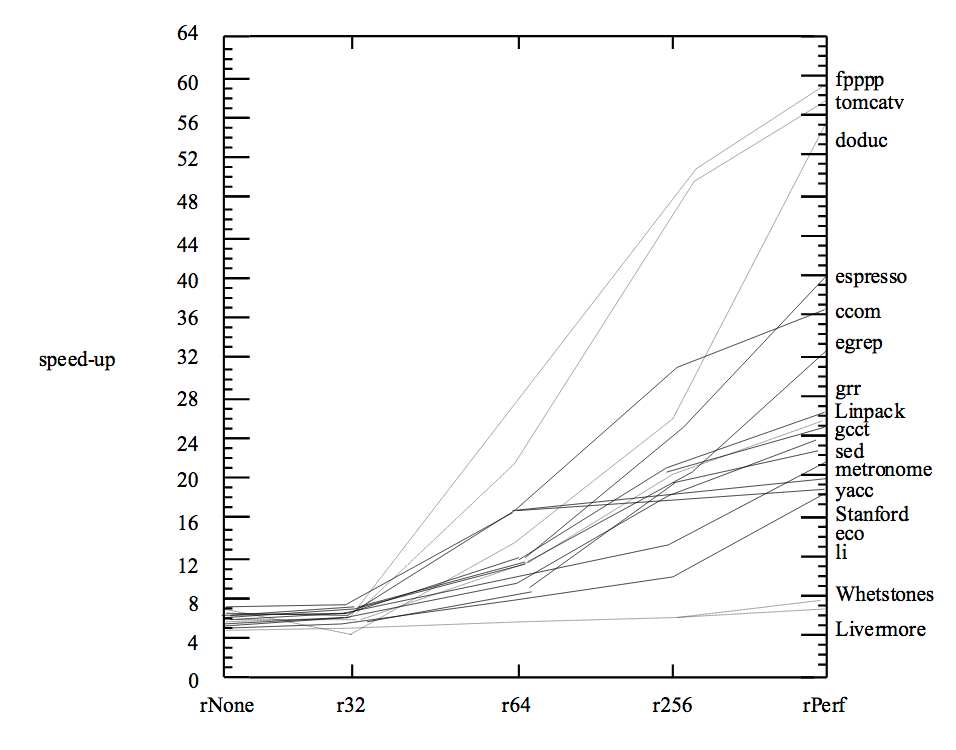
\includegraphics[width=0.7\linewidth]{figures/screenshot071}
\caption{Effects of register renaming on performance.}
\label{fig:screenshot071}
\end{figure}


Additionally, register renaming may have a significant impact. The hardware can safely \textit{rename} a register to remove a false dependency, allowing it to increase instruction-level parallelism. Algorithms for doing this have improved over the decades. This can be seen in \autoref{fig:screenshot071}, which illustrates the performance gains from the use of register renaming.
